\documentclass[12pt, twoside]{article}
\usepackage{jmlda}
\newcommand{\hdir}{.}

\usepackage{dsfont}

\usepackage{graphicx}
\DeclareGraphicsExtensions{.pdf,.png,.jpg}

\usepackage{csvsimple}

\begin{document}

\title
    [Порождение признаков с помощью локально-аппроксимирующих моделей] % краткое название; не нужно, если полное название влезает в~колонтитул
    {Порождение признаков с помощью локально-аппроксимирующих моделей}
\author
    [Максим~Христолюбов, В.\,В.~Стрижов] % список авторов (не более трех) для колонтитула; не нужен, если основной список влезает в колонтитул
    {Максим~Христолюбов, В.\,В.~Стрижов, Александра~Гальцева, Данил~Сайранов} % основной список авторов, выводимый в оглавление
    [Максим~Христолюбов, В.\,В.~Стрижов, Александра~Гальцева, Данил~Сайранов] % список авторов, выводимый в заголовок; не нужен, если он не отличается от основного
\email
    {khristolyubov.me@phystech.edu}
\thanks
    {Работа выполнена при
     %частичной
     финансовой поддержке РФФИ, проекты \No\ \No 00-00-00000 и 00-00-00001.}
\organization
    {$^1$Московский физико-технический институт}
\abstract
    {В работе рассматривается классификация временных рядов акселерометра. Классификация производится методам порождения признаков с помощью локально аппроксимирующих моделей. Предполагается, что точки временного ряда можно разбить на кластеры, соответствующие разным классам. Предлагается выделить квазипериодические сегменты из временных интервалов точек, принадлежащих одному кластеру. В качестве признаков для классификации использовать параметры моделей, обученных на этих сегментах. Исследуется вопрос информативности порожденных признаков и возможность идентификации по ним владельца прибора или его физических параметров.
	
\bigskip
\noindent
\textbf{Ключевые слова}: \emph {временной ряд; классификация; кластеризация; сегментация временного ряда; локально аппроксимирующая модель}
}

\maketitle
\linenumbers

\section{Введение}

В статье изучается задача идентификации движений человека по временным рядам. В дополнении к этому исследуется возможность выделение атрибутивных паттернов, которые могут быть использованы для определения личности или физических параметров субъектов данных в дополнении к их деятельности. Классификация временных рядов находит широкое применение в сфере здравоохранения.

Временные ряды являются объектами сложной структуры, требующие предварительной обработки и представления их в удобном для классификации виде. Необходимо отобразить исходный временной ряд в некоторое пространство признаков. Например, в статье \cite{Ivkin15} временной ряд аппроксимируется моделью, а признаками являются ее параметры. В качестве аппроксимирующей модели берется модель авторегрегрессии, а так же собственные числа траекторной матрицы, в случае модели сингулярного спектра. В работе \cite{Karasikov16} проводится разбиение временных рядов на сегменты фиксированной длины, на которых впоследствии обучается локально-аппроксимирующая модель. Для аппроксимации используется линейная модель, модель авторегрессии и коэффициенты преобразования Фурье. В \cite{Anikeev18} предлагается более разумный способ сегментации, а так же применяется аппроксимации сплайнами. Еще более общий подход к способу сегментации посредством нахождения главных компонент траекторной матрицы, рассмотрен в \cite{Motrenko16}. В \cite{Bochkarev18} сравниваются между собой перечисленные выше подходы.

Метод кластеризации точек, соответствующих участкам разной деятельности, с помощью методы главных компонента (SSA, алгоритм гусеница \cite{Danilov97}) рассмотрен в \cite{Grabovoy20}. На участках, содержащих точки одного кластера, уже можно применять описанные выше методы. Другим подходом к классификации точек временного ряда на основе нейросетей рассмотрены в \cite{Dafne19} и \cite{Cinar18}.

В работе исследуется оптимальное признаковое описание точек пр которому можно будет идентифицировать род деятельности человека. Предлагается построить набор локально-аппроксимирующих моделей и выбрать наиболее адекватные. Производится построение пространства описаний элементарных движений. Новизна работы заключается в исследовании зависимости решений задач классификации действий и предсказания параметров человека. Предположительно, эти задачи не являются не зависимыми и могут быть решены через скрытое пространство.

\section{Постановка задачи}

Пусть имеется исходный временной ряд $d=\{d_i\}_{i=1}^M\in \mathds{R}^M$. Предполагается, что он состоит из последовательности сегментов: $$d=[s_1,\ldots s_N],$$ где $s_i\in \mathcal{S}$, $|S|$~---~число различных действий (кластеров). Считается, что периоды $|s|$ сегментов различаются незначительно, причем известен максимальный период $|s|\leq T$.

Требуется решить задачу классификации точек ряда: $$R:\mathcal{I}\rightarrow Y,$$ где $\mathcal{I}=\{1,\ldots M\}$~---~индексы точек ряда, а $Y$~---~метки классов.

Кажду точку $d_k$ отобразим в временной сегмент $x_k=\{d_i\}_{i=k-T}^k$, о предположению, полностью описывающий временной ряд в окрестности точки. Это отображение зададим $$g:\mathcal{I}\rightarrow R^T$$ 

Полученные сегменты $x\in \mathcal{X}$~---~объекты сложной структуры, представленные временными рядами. Рассматривается задача классификации, а именно восстановление зависимости $$y=f(x),$$ где $y\in Y$~---~пространство ответов. Тогда исходная задача классификации представляет собой $R=f\circ g$.

Заданы выборка объектов сложной структуры и ответов $\mathfrak{D}=\{(x_i,y_i)\}_{i=1}^m$. Задача состоит в нахождении функции $f$, минимизирующие суммарные потери на выборке $\mathfrak{D}$, при заданной функция потерь $\mathscr{L}:(\mathcal{X},F,Y)\rightarrow R$, $\mathscr{L}(f(x_i),y_i)$, характеризующая ошибку классификации функции $f\in F$ на элементе $x_i$. 

Пусть $$w:\mathcal{X}\rightarrow W = \mathds{R}^n$$~---~процедура построения признакового описания сегмента. Тогда $W$~---~пространство признаков, в котором производится классификация временных рядов.

Пусть $b$~---~алгоритм многоклассовой классификации: $$b:W\rightarrow Y$$

Тогда $f$ ищется в множестве $F$ композиций вида $$f=b\circ w$$

Для любого $w$ можно найти оптимальное значение вектора $\hat\mu$ параметров классификатора $b(w(x),\mu)$, минимизирующего функционал качества: $$\hat\mu=\argmin_\mu Q(b\circ w,\mathfrak{D})$$

Оптимальный метод обучения для конкретного способа задания пространства признаков $w$ и выбранной модели классификации, определяется по скользящему контролю

$$f_{w}^*=\argmin\limits_{w}\widehat{CV}(f_{w},\mathfrak{D}),$$ где $\widehat{CV}(f,\mathfrak{D})$~---~внешний контроль качества методы обучения $f$, $\mathfrak{D}=\mathfrak{L}\sqcup\mathfrak{E}$:
 
$$\widehat{CV}(f, \mathfrak{D})=\frac{1}{r}\sum\limits_{k=1}^r Q(f^*(\mathfrak{L}),\mathfrak{E})$$

В качестве функционала качества используется $$Q(f,\mathfrak{L})=\frac{1}{|\mathfrak{L}|}\sum\limits_{(x,y)\in\mathfrak{L}}|\{(x,y)\in\mathfrak{L}|f(x)=y\}|$$, а в оценке точности классификации объектов класса $c\in Y$ используется модифицированный функционал качества $$Q_c(f,\mathfrak{L})=\frac{1}{|\mathfrak{L}|}\sum\limits_{(x,y)\in\mathfrak{L}}\frac{|\{(x,y)\in\mathfrak{L}|f(x)=y=c\}|}{|\{(x,y)\in\mathfrak{L}|y=c\}|}$$


\section{Порождение признаков}

Модели, с помощью которых производится порождение признаков временных сегментов, называются локально-аппроксимирующими моделями, в силу локальности рассматриваемого сегмента временного ряда. В качестве признаков сегмента предлагается брать вектор оптимальных параметров $w$ локально-аппроксимирующими модели $M$: $$w_M(x)=\argmin\limits_{w}\rho(M(w,x),x).$$

При работе с многомерным временным рядом можно применить операцию порождения признакового описания в точке к каждому одномерному ряду, а потом объединить все полученные признаки.


\subsection{Авторегрессия}
Модель авторегрессии $AR(T)$ предсказывает следующее значение временного ряда как линейную комбинацию $T$ предыдущих.
$$\hat x^{(k)}=w_0+\sum\limits_{i=1}^T w_i x^{(k-i)}$$

Для нахождения оптимального вектора параметров нужно решить задачу минимизации (при евклидовом расстоянии между рядами):
$$w_M(x)=\argmin_w(||x-\hat x_M||_2^2=\argmin_w||x-Xw||_2^2=(X^TX)^{-1}X^Tx$$

\begin{equation*}
X = \left(
\begin{array}{cccc}
x^{(1)} & x^{(2)} & \ldots & x^{(T)}\\
x^{(2)} & x^{(3)} & \ldots & x^{(T+1)}\\
\vdots & \vdots & \ddots & \vdots\\
x^{(2T+1)} & x^{(2T+2)} & \ldots & x^{(3T)}
\end{array}
\right)
\end{equation*}

\subsection{ Анализ сингулярного спектра}
Рассмотрим модель SSA порождения данных. Поставим в соответствие временному сегменту $x$ траекторную матрицу $X$. Ее сингулярное разложение $$X^TX=VHV^T, H = diag(h_1,\ldots h_T).$$ $h_1\ldots h_T$~---~собственные числа матрицы $X^TX$ берутся в качестве нового признакового описания $w=h$. Они отвечают за величины различных частот спектра $x$.

\subsection{ Дискретное преобразование Фурье}
К временному сегменту можно применить дискретное преобразование Фурье:
$$w_k = \sum\limits_{n=1}^{T-1}x_n^ke^{-\frac{2\pi i}{T}kn}$$
и взять в качестве признаков $w$ его коэффициенты.


\section{Вычислительный эксперимент}

Данные для эксперимента представляют собой измерения акселерометра и гироскопа, встроенных в мобильное устройство IPhone 6s, хранящегося в переднем кармане брюк участника. Временные ряды содержат значения ускорения человека и углы ориентацию телефона для каждой из $3$ осей~---~всего $6$ временных рядов. Частота дискретизации составляет $50$ Гц. Метками классов служат: подъем по лестнице вверх, спуск по лестнице вниз, ходьба, бег трусцой, сидение, лежание. Данные собраны с $24$ участников, для каждого из  которых известны рост, вес, возраст и пол. Данные собирались в условиях проведения эксперимента: участникам выдавали телефон и просили выполнять одно из $6$ действий в течении $1-2$ минут.

Для эксперимента берется $6$ временных рядов в $39000$ точек ($780$ секунд). Данные снимаются с $4$ человек ($2$ мужчины и $2$ женщины), которые выполняют подъем или спуск по лестнице ($2$ типа деятельности).

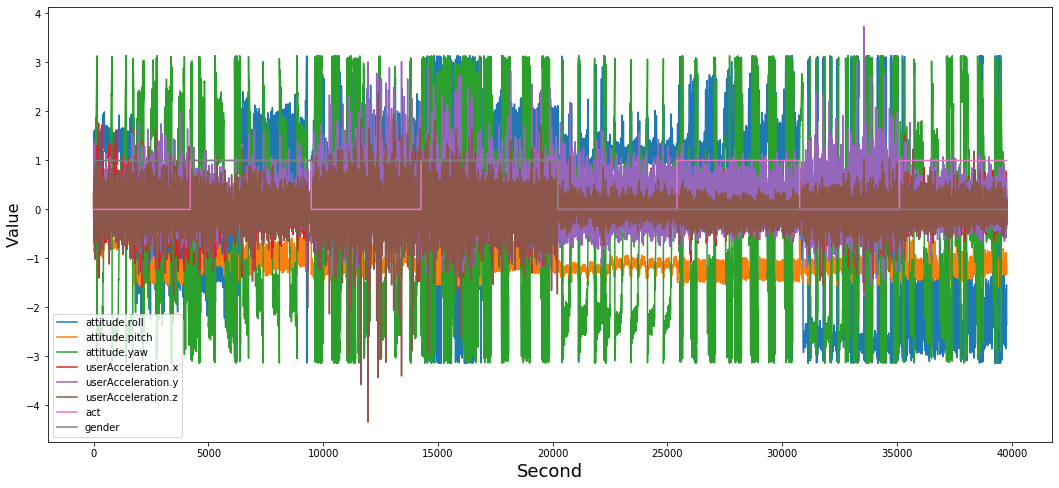
\includegraphics{data}

В силу большой размерности и того, что тип деятельности не меняется часто, целесообразно не классифицировать каждую точку временного ряда (которых в $1$ секунде $50$ штук), а с каким то шагом, а остальные точки относить к тому же классу, которому принадлежит ближайшая точка. Это позволяет уменьшить размер выборки для классификации с $39000$ точек до $3900$, если классифицировать каждую десятую точку.

На соответствующих точкам сегментах строятся локально-аппроксимирующие модели, чьи параметры используются в качестве признаков. Сравниваются информативность признаков, порожденных моделью авторегресси (с $50$ членами), коэффициенты ряда Фурье ($100$ для каждого ряда), $50$ сингулярных чисел SSA разложения. 

Отбор оптимальныхпризнаков производится сначала по критерию Пирсона (остается $96$ признаков), потом оптимальные $20$ методом перебора Sequential Backward Floating Selection для выбранной модели классификации. Рассматриваются модели Logistic Regression и C-Support Vector Classification. 

Для исследования зависимости между решением задач классификации активности и гендера находятся общие признаки, попавшие в векторы оптимальных параметров для решения обоих задач классификации. Однако, в силу высокой размерности
и мультиколлинеарности возможна ситуация, когда для решения обоих задач используют одну и ту же информацию, хотя векторы оптимальных признаков не имеют общих компонент. Поэтому для проверки наличия причинно-следственной зависимости между активностью и гендером производится обучения на расширенной матрице признаков: сначала решается одна задача классификации, а потом полученный вектор решения используется как признак для решения второй задачи.

\csvautotabular{../data/result.csv}

Таким образом, предварительное определение гендера улучшает классификацию движения, а предварительное определение движения ухудшает классификацию гендера. Отсюда можно сделать предположение о том, что имеет место причинно-следственная связь: гендер влияет на тип активности, что соответствует эмпирическим представлениям.



\section{Заключение}
Желательно, чтобы этот раздел был, причём он не~должен дословно повторять аннотацию.
Обычно здесь отмечают, каких результатов удалось добиться, какие проблемы остались открытыми.

%%%% если имеется doi цитируемого источника, необходимо его указать, см. пример в \bibitem{article}
%%%% DOI публикации, зарегистрированной в системе Crossref, можно получить по адресу http://www.crossref.org/guestquery/
%\begin{thebibliography}{99}
	
 	
%\end{thebibliography}

\maketitleSecondary
\English
\begin{thebibliography}{99}

\bibitem{Ivkin15}
	\BibAuthor{N.~P.~Ivkin, M.~P.~Kuznetsov.}. 2015.
	 Time series classification algorithm using combined feature description. .
	\BibJournal{Machine Learning and Data Analysis} (11):1471–1483.

\bibitem{Karasikov16}
	\BibAuthor{V.~V.~Strijov, M.~E.~Karasikov.} 2016.
	Feature-based time-series classification
	\BibJournal{Informatics}
	\BibDoi{10.3114/S187007708007}.
	
\bibitem{Anikeev18}	
	\BibAuthor{D.A. Anikeev, G.O. Penkin, V.V. Strijov}. 2018.
	Local approximation models for human physical activity classification~//
	\BibJournal{Informatics}
	\BibDoi{10.14357/19922264190106}.

\bibitem{Isachenko16}
	\BibAuthor{V.V. Strijov, R.V. Isachenko.}. 2016.
	 Metric learning in multiclass time series classification problem.
	\BibJournal{Informatics and Applications} (10(2)):48–57.

\bibitem{Popova16}
	\BibAuthor{V.V. Strijov, Andrew~Zadayanchuk, Maria~Popova.}. 2016.
	 Selection of optimal physical activity classification model using measurements of accelerometer.
	\BibJournal{Information Technologies}  (22(4)):313–318.

\bibitem{Motrenko16}
	\BibAuthor{Strijov~V.V., Motrenko~A.P.}. 2016.
	 Extracting fundamental periods to segment human motion time series.
	\BibJournal{Journal of Biomedical and Health Informatics}  20(6):1466 – 1476.

\bibitem{Ignatov15}
	\BibAuthor{Strijov~V.V., Ignatov A.}. 2015.
	 Human activity recognition using quasiperiodic time series collected from a single triaxial accelerometer.
	\BibJournal{Multimedia Tools and Applications}  pages 1–14.
	
\bibitem{Bochkarev18}
	\BibAuthor{Isachenko R.V., Bochkarev А.М., Zharikov I.N., Strijov V.V.}. 2018.
	Feature Generation for Physical Activity Classification.
	\BibJournal{Artificial Intelligence and Decision Making}  3 : 20-27.

\bibitem{Dafne19}
	\BibAuthor{Dafne van Kuppevelt, Joe Heywood, Mark Hamer, Séverine Sabia, Emla Fitzsimons, Vincent van Hees}. 2019.
	 Segmenting accelerometer data from daily life with unsupervised machine learning.
	\BibJournal{PLOS ONE}
    \BibDoi{10.5255/UKDA-SN-8156-3}.
    
\bibitem{Sabatini10}
    \BibAuthor{Andrea Mannini, Angelo Maria Sabatini}. 2010.
    Machine Learning Methods for Classifying Human Physical Activity from On-Body Accelerometers
    \BibJournal{PubMed}
    \BibDoi{10.3390/s100201154}.
    
\bibitem{Grabovoy20}
	\BibAuthor{Grabovoy A.V., Strijov V.V}. 2020.
	Quasiperiodic time series clustering for human activity recognition
	\BibJournal{Lobachevskii Journal of Mathematics}
	
\bibitem{Danilov97}
	\BibAuthor{D.L. Danilov and A.A. Zhiglovsky}. 1997.
	\BibTitle{Main components of time series: method "Gesenitsa" (St. Petersburg)}
	
\bibitem{Cinar18}
	\BibAuthor{ Y.G. Cinar and H. Mirisaee}. 2018.
	Period-aware content attention RNNs for time series forecasting with
	missing values
	\BibJournal{”Neurocomputing}  312, 177–186
    
\bibitem{Malekzadeh19}
	\BibAuthor{Malekzadeh, Mohammad and Clegg, Richard G. and Cavallaro, Andrea and Haddadi, Hamed}. 2019.
	\BibTitle{Mobile Sensor Data Anonymization}  pages 49--58.
    \Bibbooktitle{Proceedings of the International Conference on Internet of Things Design and Implementation}
    \BibDoi{10.1145/3302505.3310068}.
 

\printbibliography
  	     	
\end{thebibliography}

\end{document}
